\documentclass[10pt]{article}

\usepackage{graphicx}

\begin{document}

\title{Coordinating parallelism between build systems and compilers to improve scalling on multi-core machines}
\author{Sarah Spall}
\date{}
\maketitle

\section{Introduction}

In today's world multi-core machines are ubiquitous, with machines having up to 64 physical cores.
Having a machine with 64 cores instead of 32 cores isn't useful however, if the software running
on it isn't capable of utilizing the 32 additional cores.  Unfortunately, while extensive effort
has gone into optimizing a wide variety of domains; build systems and compilers remain
neglected. Even though every developer
uses a build system and a compiler, they still do not scale to modern many-core systems.

% What is the high level thing I want to say?
The build systems and compilers of today tend to work separately even though they solve
separate parts of the same problem.  The build system is usually responsible for coordinating
thes sequential tasks that make up a project build; these sequential tasks are often
compilation jobs.  On the other hand, the compiler is responsible for completing many of the sequential
tasks that the build system is waiting on.  Traditionally, independent compilation jobs can be
launched in parallel by the build system if they do not depend on one another, but internally,
most modern compilers do not themselves run in parallel.

I propose the following thesis: \emph{By combining and coordinating parallelism between the build system level
and the compiler level, project builds can better scale on modern day multi-core
machines.}

In support of this thesis I propose three separate lines of research.  First, I will analyse the parallelism
currently exposed and observed in existing projects.  Second, I will investigate ways to expose
additional parallelism at the build system level.  Third, I will show how to improve the
parallelism of compilers, and show that a parallel compiler can work
in concert with a build system to better exploit available parallelism.  The following
sections of this proposal explain in more detail how I plan to accomplish these goals.

\section{The current state of parallel builds}
\label{sec:state}
% Start out talking about multiple build systems and how they general all work
% Then move onto the specifics of Make itself.

% List of build systems: Make, Shake, Bazel, Buck, Ninja, 

There are many existing build systems whose general goal is to build a project efficiently
including, Make \cite{feldman1979make}, Shake
\cite{mitchell2012shake}, Bazel \cite{bazel}, Buck \cite{buck}, and Ninja \cite{ninja}.
All of these build systems will launch independent tasks in parallel as one method of building a
project as quickly as possible.

Most build systems use a dependency graph to decide the correct  order to launch jobs and which jobs are
independent from one another.  If two or more jobs are independent they can be executed
in parallel.  Therefore, a dependency graph describes the obvious parallelism available in a project build
and makes it easy for a build system to exploit it.

Make is a ubiquitous build system that first uses the information specified  in a
Makefile to construct a directed graph of a build project's tasks.  Make then performs a
topological sort on the graph to determine the order to build the targets.  Programmers can
specify which tasks
for a specific target may safely be run in parallel by specifying them as dependencies of the
target, or by writing a line such as \emph{make one two three}.  Make lets users specify how many
jobs may run at once, but of course how many jobs will run in parallel is directly dependent on the amount
of parallelism available in the project's directed graph.   We would like to go
beyond this model of build-level parallelism and discover more parallelism within the compilation jobs
launched by the build system.

Buck appears to go beyond this model of exploiting only the obviously available parallelism.  
Usually it is entirely the user of the build system's job to fully define which tasks are independent.
Buck claims to not require users to fully define which tasks are independent and will break coarse-build rules
up into smaller independent pieces that can be built in parallel.  

% not sure if this note about shake really fits here
%shake has an interesting strategy for reducing contention for system resources such as IO and
%memory; which is to run tasks in a random order.  They believe that it is more likely that tasks
%which are close together are more likely to use the same system resources.

% Make lets users to -j n; so can build independent targets in parallel; where the independence
% of any number of targets is defined by the user.

% Shake is the haskell build system which..... also allows independent rules at the same time
% shake has a thread pool and rules are added to a queue to be run by the thread pool.
% which I believe is just about the same as Make and probably every system
% user can specify max number of rules run in parallel
% shake says it ensures max parallelism by launching a temporary worker when a rule is blocked
% waiting on dependencies; why does this ``ensure'' max parallelism?
% run tasks in a random order to reduce contention for system resources

% bazel is google's build system
% says you can set it up to run ``in a highly parallel and incremental fashion''
% bazel has a -j option which says it allows the user to specify the number of jobs that should
% be executed CONCURRENTLY; the scheduler tries to avoid running more concurrent jobs if
% it will negatively affect resource usage 
% bazel claims it allows builds to scale by caching and remote execution.
% What do they mean by scale?  To larger and larger projects?  Prob don't mean scale to use
% many many cores

% buck is facebook's build system
% buck says it constructs a DAG and then can easily know what can be built in parallel;
% like make
% Buck acknowledges this fact ``This execution model means that breaking modules into finer
% dependencies creates opportunities for increased parallelism, which improves throughput.''
% buck uses something they call ``graph enhancement'' to expose more parallelism
% graph enhancement can break up a larger task into smaller ones that can be done in parallel
% graph enhancement can also move dependnecy edges.
% not sure what kind of analysis they do to determine this; maybe its very shallow or very
% intelligent
% should look at source code
% action graph is only built once; unless dependencies in buid file change

% ninja; built by some guy at google?
% builds are always run in parallel; so just like every other project.  by default

% talk about parallel compilation now
% need to say more


% Why didn't these things make it into production compilers?

% maybe the following sentence belongs in the next section?
%It is generally considered difficult to write good parallel programs, so much work has gone into
%providing developers with tools for analysing the parallelism in their programs [citations].  

% say how builds create a graph then run things in parallel based on dependency info
% but most of those tasks being run are sequential processes


% I should probably validate the above claim

% want to go beyond this model

% Ask ryan about using his 1 versus 16 core debian build parallelism

\begin{figure}[t]
  \centering
  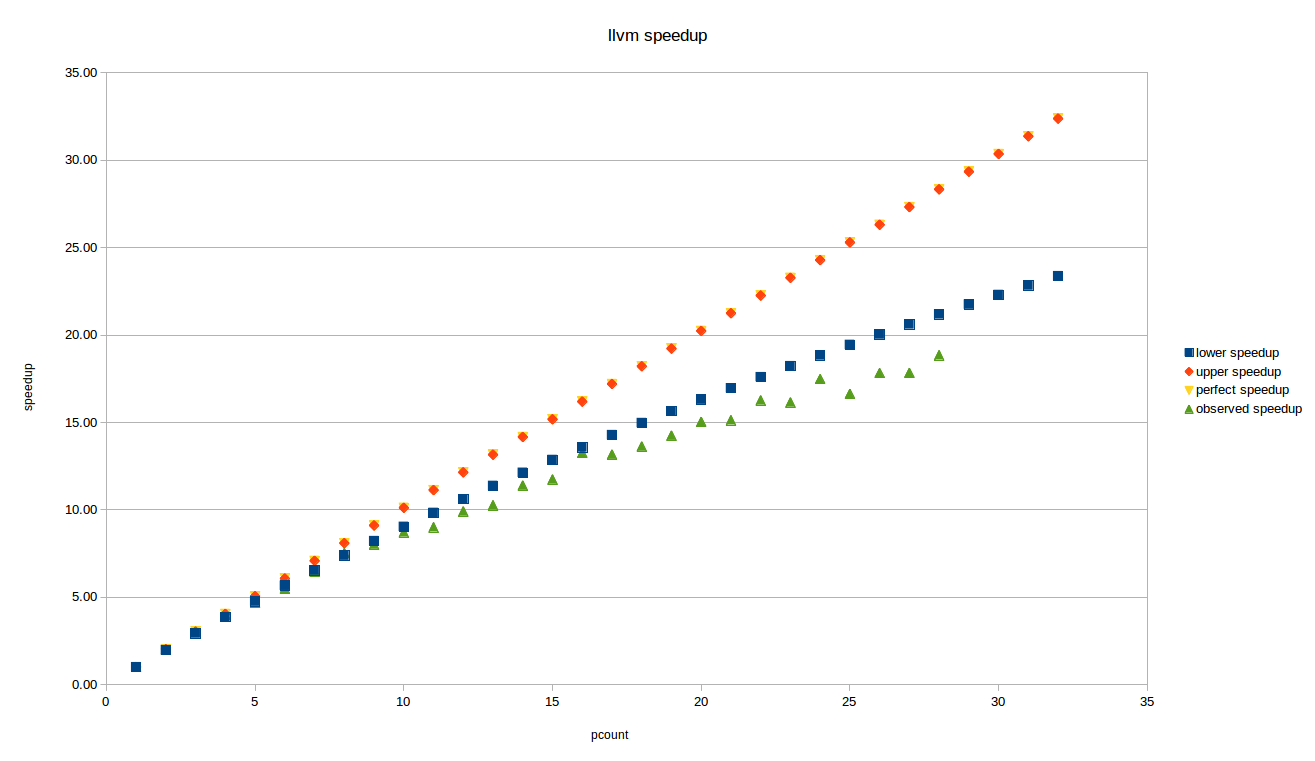
\includegraphics[height=6.2cm]{llvm-speedup-chart.png}
  \caption{Building LLVM on 1 to 28 cores.}\label{fig:llvm}  % update this with to 32 cores
\end{figure}

\begin{figure}[t]
  \centering
  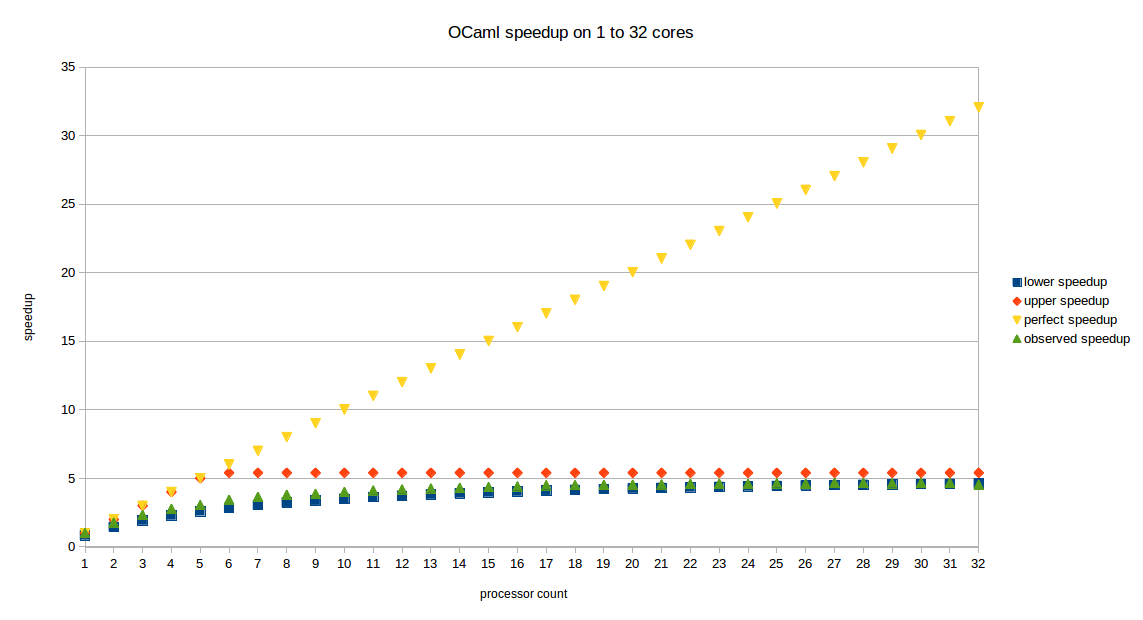
\includegraphics[height=6.2cm]{ocaml-speedup-chart.png}
  \caption{Building Ocaml on 1 to 32 cores.}\label{fig:ocaml}
\end{figure}

We have already begun to analyse the parallelism in project builds that use Make.  Two
project builds we have already analysed are LLVM \cite{llvm} and OCaml \cite{ocaml}.
LLVM is a very large project that has been observed to take about 3.4 hours to build on a
single core.  See figure~\ref{fig:llvm} on page~\pageref{fig:llvm} to see how the LLVM build scaled
when built on 1 to 32 cores.  This chart also shows the predicted upper speedup and lower speedup bounds, as
calculated by Brent's law \cite{brent1974parallel}.  These predictions were calculated using a
parallel analysis tool for Make that is described in section \ref{sec:build}.  LLVM's build has
a parallelism of about 82, which means we would expect it to scale close to perfectly on 32 cores.
As we see in the chart, the speedup gained by more cores flattens substantially at about 24 cores.
We predict this failure to scale as well as possible is due to contention for system resources.


OCaml is a smaller project that has been observed to take about 2.6 minutes to build on a single core.
In figure~\ref{fig:ocaml} on page~\pageref{fig:ocaml} to see how the OCaml build scaled when built
on 1 to 32 cores.  Unlike with LLVM, OCaml's build does not expose ample parallelism for 32 cores and
has a parallelism of about 7.  For builds that exhibit low levels of parallelism, we would like to
expose more parallelism by reducing the span of the project, which for OCaml's build is about 20 seconds,
or running sequential compilation jobs in parallel.


Even though almost all production compilers are not parallel, research
has been done on how to parallelize certain compiler passes.  These passes include
parsing \cite{barenghi2015parallel}, register allocation \cite{makowski1995achieving} \cite{zobel1993program}, program analysis \cite{kuper2014freeze}
\cite{mendez2010parallel} \cite{prabhu2011eigencfa} \cite{zobel1992program}, and typechecking \cite{newton2016parallel}.
This work probably has not made it into many mainstream compilers due to the general difficulty of writing
performant parallel programs, and the complicated algorithms and data structures used to write compilers.

\section{Parallel analysis tool for build systems}
\label{sec:build}

A project build is just a specialized parallel program, but not much effort has gone
into helping developers write builds that are as parallel as possible.  Many, parallel
analysis tools have been created that help programmers optimize general parallel programs,
such as, Cilkprof \cite{schardl2015cilkprof}, Kremlin \cite{garcia2011kremlin}, and TaskProf
\cite{yoga2017fast}.

To the best of my knowledge, there is no parallel analysis tool for project builds, and in the
spirit of previous parallel analysis tools, I propose such a tool for Make.  This tool will
serve two main purposes; first, it will help us analyse and understand the current state of
parallelism in project builds using Make, and second, it will assist programmers in their project
builds and will be able to make suggestions of which targets and rules could be rewritten to
expose more parallelism.

Work has already begun on this tool and it has been used to analyse the builds of
projects such as LLVM \cite{lattner2002llvm} and OCaml \cite{ocaml}.  The tool works by
recording information from a run of GNU Make and then reconstructing the build's DAG
during a post-mortem analysis of the run.  With this we can perform an analysis similar
to other parallel analysis tools and calculate values such as work, span, and
parallelism.
Additionally we can record all of the system calls made during the course of the build.
From this we can determine all of the files used by each shell command run during the build, and
can state at a file-level whether one shell-command potentially depends on another shell-command.
This will let us determine the accuracy of user defined dependencies.
% brief overview of how these 3 tools work.

\section{Parallel compilers}

% parallelizing compilers; gibbon paper; better representations for parallelizing compilers
% paralle lvars?

% Move on to parallel compilers and the lack of parallel compilation.....  Still need to motivate
% this and I suppose the build stuff
Many of the long sequential tasks launched by a build system are compilation jobs.  Thus, to
expose additional parallelism beyond what can be exposed at the build system level, an at least
partially parallel compiler is necessary.  A parallel compiler could decrease the span
of a previously sequential task and thus potentially decrease the span of the project build as a
whole.  Additionally, for projects that are failing to scale as well as their available parallelism
predicts they should, it may prove useful to move some of that parallelism to a different area.
For example, maybe 16 threads all reading different files is putting too much pressure on the file
system and causing excessive overhead, but having 4 groups of 4 threads operate on 4 different files
in parallel, might increase observed parallelism by decreasing resource contention.

% Certainly what Shake does is also work considering doing but I'm not sure best way to work that in atm

To validate this hypothesis we can measure the utilization of various system resources when
a representative project is built with exclusively build-level parallelism and when a
the same project is built with a mix of build-level and compilation-level parallelism.  Resource utilization
could then be compared to predicted speedups and observed speedups.  If moving soe of the parallel work
to the compilation-level releaved contention, we would expect to see lower resource utilization for the
seconds benchmark for some resources, as well as increased observed parallelism.

% should I explain what different results owuld mean?

In section \ref{sec:state} I mentioned previous work that has been done on parallelizing various compiler
passes and here I will discuss some work we have already done in this direction. 

In our work on the Gibbon compiler \cite{vollmer2017compiling}, we showed that transforming trees into a serialized
format and transforming the code that operates on those tres to operate on the serialized format,
results in a major performance improvement.  We believe this serialized tree format could be used to
write parallel compiler passes.  When the parallel version of a Gibbon benchmark was compared to
GHC running the same parallel benchmark, it was observed that for large trees, a speedup of
11x was observed on 16 cores when compared to a sequential execution.  And, it was observed that GHC
failed to scale beyond 8 cores due to time spent in the garbage collector.  Due to the speedup from
the serialization format itself and the lessened demands on memory allocation we believe Gibbon
could be used to write a performant parallel compiler pass.

% probably butchered that explanation

\section{Scheduler for coordination between build system and compilers}

When exploiting parallelism at both the build-level and at the compiler-level, it may be possible to
decrease observed parallelism by launching too many processes or threads.  In order for the build
system and the compiler to work together as one, a scheduler with a view of the entire system
is necessary.  This scheduler should detect when it is appropriate to run parallel compilation
jobs, and when there is enough parallelism available at the build level to make that unnecessary.
There are of course additional things that could be taken into account, such as: information about which
paths contributed to the span in previous runs could help determine how
to distribute the parallelism in future runs.
For example, Maybe compiling file B takes x
seconds, and would take half that time if parallelized, but if compiling x didn't contribute to
the overall span, then there would be no observed benefit from running that task in parallel.

\section{Conclusion}

In conclusion, I propose the following thesis: \emph{By combining and coordinating parallelism at the build system level
and at the compiler level, project builds can better scale on modern day multi-core
machines.}  And, in support of this thesis I propose analysing and improving the parallelism available in Make builds,
discovering methods for parallelizing compiler passes, and showing that with a scheduler to coordinate parallelism at
the build-level and compiler-level project builds can scale better on modern multi-core machines.

\newpage
\bibliography{citations}
\bibliographystyle{ieeetr}

\end{document}
